\chapter{Segranks - Experiments With The Database of Annotations}

In this chapter we describe several experiments with the collected database of
annotations. 

\section{Overall Ranking of Annotated Systems}
\label{evaluating-annotated-systems}

In the first experiment we would like to show that the proposed method can be
used to produce overall ranking of the annotated systems which will be very
similar to the official human evaluation in WMT with much less human effort
\XXX{dolozit, pokud je to vubec pravda a pokud to vubec pujde}.

The obtained database contains a list of annotations for each extracted source
segment from each source sentence. A list can be empty (not all of the
sentences were annotated), it can contain more than one annotation (some
segments were annotated twice by an annotator, some segments were annotated by
multiple annotators), but most of the time it contains only one annotation.

An annotation is a mapping from the set of candidate segments to the set of
ranks ${1 \ldots N+1}$, where $N$ is the count of unique candidate segments.
(To discriminate the relative quality of all segments, annotators had available
$N$ ranks which could be all occupied when there are no ties. The rank $N+1$
represents the ``garbage'' category from the annotation application. However in
all of our experiments reported in this thesis we consider this category as one
more, the worst, rank). A Lower rank of a segment means that the candidate
segment was ranked better. This is an example \metoda{segment annotation} of a
source segment ``the huge volume'':

\begin{verbatim}
    {
      'velkému objemu' : 1,
      'obrovské hlasitosti' : 5,
      'obrovský objem' : 2,
      'obrovské množství' : 2,
    }
\end{verbatim}

We expanded these segment annotations with the information about the systems
which produced the segments. The ranks in the annotations are now indexed by
the system names.  If more systems translated a source segment as the same
candidate segment the candidate segment's rank is copied to all the systems.
This is the time when we use advantage of ranking short segments which are
often translated identically.  The following is the \metoda{system annotation}
after expansion of the above \metoda{segment annotation}:

\begin{verbatim}
    {
      'uedin-unconstrained' : 2,
      'commercial1' : 5,
      'commercial2' : 2,
      'CU-TectoMT' : 1,
      'onlineB' : 2,
      'onlineA': 2,
      'cu-funky' : 2,
      'cu-bojar' : 2,
      'uedin-wmt14': 2,
      'cu-depfix': 2
    }
\end{verbatim}

These rankings are now very similar to those obtained in the official WMT human
evaluation. These annotations are mostly interpreted as pairwise systems'
comparisons (for each combination of size 2 of all systems we have a pairwise
comparison), where the absolute values of the ranks and their absolute
differences between them are not considered. From above \metoda{system
annotation}, the following \metoda{pairwise comparisons} are be extracted (only
a few extracted pairwise comparisons are listed here for the sake of brevity,
generally $N \times (N-1) / 2$ pairwise comparisons are extracted, where $N$ is
number of all systems):

\begin{verbatim}
    [
      'uedin-unconstrained' < 'commercial1',
      'uedin-unconstrained' = 'commercial2',
      'uedin-unconstrained' > 'CU-TectoMT',
      ...
      'commercial1' > 'commercial2',
      'commercial1' > 'CU-TectoMT',
      ...
    ]
\end{verbatim}

The interpretation of these pairwise comparisons was changed several times
during the WMT workshops. Here, we use \metoda{Ratio of wins (ignoring ties)}
method, which was introduced by \perscite{bojar:grain:of:salt} and used in
WMT12 workshop \parcite{callisonburch:wmt12}. This method is based on a method
used in several WMT workshops before WMT12 and it is quite easy to compute and
interpret results.

For a given set $C$ of segment-level extracted pairwise comparisons
$(s_1,s_2,c)$, where 

\begin{equation*}
c = \begin{cases}
  win  & \text{if $rank(s_1) < rank(s_2)$} \\
  loss & \text{if $rank(s_1) > rank(s_2)$} \\
  tie  & \text{if $rank(s_1) = rank(s_2)$} \\
    \end{cases}
\end{equation*}

\noindent we define for each system $s$ the total number of wins, losses and ties:

\begin{equation*}
\begin{array}{rcl} 
  win(s)  & := & |\{(s,\bar{s},c) \in C; c = win\}| + |\{(\bar{s},s,c) \in C; c = loss\}| \\
  loss(s) & := & |\{(s,\bar{s},c) \in C; c = loss\}| + |\{(\bar{s},s,c) \in C; c = win\}| \\
  ties(s) & := & |\{(s,\bar{s},c) \in C; c = tie\}| + |\{(\bar{s},s,c) \in C; c = tie\}| \\
\end{array}
\end{equation*}

Then the \metoda{Ratio of wins (ignoring ties)} for a given system $s$ is
computed using the following formula:

\begin{equation*}
  E_{win}(s) = \frac{win(s)}{win(s) + loss(s)} 
\end{equation*}

\begin{table}
  \begin{center}
    \subfloat[Short segments judgements]{
      %\begin{center}
        \begin{tabular}{|l|c|}
          \hline
          \textbf{System} & \textbf{Score} \\
          \hline
           cu-depfix           &  0.5777 \\
           onlineB             &  0.5642 \\
           uedin-unconstrained &  0.5626 \\
           cu-bojar            &  0.5606 \\
           cu-funky            &  0.5566 \\
           uedin-wmt14         &  0.5498 \\
           onlineA             &  0.5007 \\
           CU-TectoMT          &  0.4485 \\
           commercial1         &  0.3992 \\
           commercial2         &  0.3492 \\
          \hline
        \end{tabular}
      %\end{center}
      \label{all-systems-segranks-results}
    }
    \subfloat[Official WMT14 judgements]{
      %\begin{center}
        \begin{tabular}{|l|c|}
          \hline
          \textbf{System} & \textbf{Score} \\
          \hline
          cu-depfix          &  0.6101 \\
          cu-bojar           &  0.6011 \\
          uedin-unconstrained&  0.5967 \\
          cu-funky           &  0.5823 \\
          onlineB            &  0.5439 \\
          uedin-wmt14        &  0.5285 \\
          onlineA            &  0.5039 \\
          CU-TectoMT         &  0.4473 \\
          commercial1        &  0.3617 \\
          commercial2        &  0.2780 \\
          \hline
        \end{tabular}
      \label{all-systems-wmt-results}
    }

  \end{center}

  \caption[Overall system rankings computed on short segment judgments]{Overall
    rankings of systems according to \metoda{Ratio of wins (ignoring ties)}
    score. You can see the results computed on both short segments judgements
    and on official WMT14 human judgements side by side to compare the
  differences.}

  \label{all-systems-results}
\end{table}

\subsection{Results}

The overall ranking of systems, which participated in WMT14 Translation Task in
English-Czech direction, according to the \metoda{Ratio of wins (ignoring
ties)} computed on the short segments judgements is reported in the table
\ref{all-systems-segranks-results}.

To compare our method with the classic method of judging whole sentences, we
have also computed the \metoda{Ratio of wins (ignoring ties)} on the judgements
collected during WMT14 manual evaluation. You can see these results in the
table \ref{all-systems-wmt-results}.

You can notice that the range of scores computed on the short segments
judgements is much narrower (0.35 --- 0.58) than the range of scores computed
on the sentence judgements (0.28 --- 0.61). This can be explained by the
following: If system A beats system B in a sentence-level judgement of a
particular sentence it does not necessarily mean that in segment-level judging
system A will be better than system B on all segments of the sentence. System A
will be probably better on a majority of the segments (but even that does not
have to be always true). When computing the ratio of wins on the sentence-level
judgements, system A gets one win and system B gets one loss. However, when
computing the ratio of wins on the segment-level system A gets for example two
wins and one loss, system B one win and two losses. It should be clear now that
computing expected wins on the sentence-level judgements is coarser while our
method is more fine-grained.  \XXX{Co z toho vlastne plyne? Je to dobre, nebo
spatne?}

The overall rankings of systems obtained by both of the methods is very
similar. However, there are two changes when comparing to the sentence-level
judgments results: system online-B is better and system cu-bojar is worser
according to the segments-level judgments results. We try to explain this in the Analysis.

\subsection{Analysis}

To see the difference between the segment-level judgements and sentence-level
judgements we have computed Kendall tau rank correlation coefficient, also
known as Kendall's $\tau$, between segment-level pairwise comparisons and
sentence-level pairwise comparisons. This coefficient is used to measures how
often a set of pairwise rankings agrees with another set of pairwise rankings.
The basic formula for Kendall's $\tau$ is:

\begin{equation*}
  \tau = \frac{|Concordant| - |Discordant|}{|Concordant| + |Discordant|}
\end{equation*}

\noindent where $Concordant$ is the set of pairwise combination where both sets
of pairwise rankings agrees with each other and $Discordant$ is the set of
pairwise combination where the sets do not agree in pairwise ranking.
\XXX{mozna vyhodit predchozi vetu}  We will discuss the Kendall's $\tau$ in
more details in chapter \ref{metrics}. Here we computed $|Concordant|$ as the
number of pairwise segment-level judgments which agrees with the corresponding
sentence-level judgment. Similarly, $|Discordant|$ is the number of those which
does not agree with the corresponding sentence-level judgment. In this section
we does not consider any tied pairwise comparisons.

\begin{table}
  \begin{center}
    \subfloat[Better systems]{
      %\begin{center}
        \begin{tabular}{|l|c|}
          \hline
          \textbf{System}                   &   $\tau$ \\
        \hline
         cu-funky            &        0.428 \\
         cu-depfix           &        0.405 \\
         onlineB             &        0.398 \\
         cu-bojar            &        0.394 \\
         uedin-uncon. &        0.390 \\
         uedin-wmt14         &        0.363 \\
         onlineA             &        0.312 \\
         CU-TectoMT          &        0.270 \\
         commercial1         &        0.166 \\
         commercial2         &        0.123 \\
          \hline
        \end{tabular}
      %\end{center}
      \label{sentence-segments-judgments-correlations-better}
    }
    \,
    \subfloat[Worse systems]{
      %\begin{center}
        \begin{tabular}{|l|c|}
          \hline
          \textbf{System}                   &   $\tau$ \\
       \hline
         commercial2         &        0.492 \\
         commercial1         &        0.441 \\
         CU-TectoMT          &        0.385 \\
         onlineA             &        0.328 \\
         uedin-uncon. &        0.260 \\
         uedin-wmt14         &        0.257 \\
         cu-funky            &        0.230 \\
         cu-bojar            &        0.227 \\
         cu-depfix           &        0.225 \\
         onlineB             &        0.225 \\
          \hline
        \end{tabular}
      \label{sentence-segments-judgments-correlations-worse}
    }
    \,
    \subfloat[All systems]{
      %\begin{center}
        \begin{tabular}{|l|c|}
          \hline
          \textbf{System}                   &   $\tau$ \\
        \hline
         commercial2         &        0.394 \\
         cu-funky            &        0.348 \\
         commercial1         &        0.345 \\
         uedin-uncon. &        0.341 \\
         cu-depfix           &        0.335 \\
         CU-TectoMT          &        0.333 \\
         cu-bojar            &        0.328 \\
         onlineB             &        0.321 \\
         onlineA             &        0.320 \\
         uedin-wmt14         &        0.317 \\
          \hline
        \end{tabular}
      \label{sentence-segments-judgments-correlations-all}
    }

  \end{center}

  \caption[Correlations between the segment-level judgments and sentence-level
  judgments]{Kendall's $\tau$ correlations between the segment-level and
    sentence-level judgments. For a given system we computed the correlation on
    all pairwise comparisons including the given system. The table
    \ref{sentence-segments-judgments-correlations-better} contains correlations
    computed on sentence-level judgments where the given system was better, the
    table \ref{sentence-segments-judgments-correlations-worse} is computed on
    sentence-level comparisons where the given system was worse and finally the
    table \ref{sentence-segments-judgments-correlations-all} was computed on
    all pairwise comparisons including the system. The systems are sorted by
    the correlation in reverse order.} 

  \label{sentence-segments-judgments-correlations}
\end{table}

The computed correlations are tabulated in the table
\ref{sentence-segments-judgments-correlations}. The order of the systems in the
table \ref{sentence-segments-judgments-correlations-better} is quite similar to
the order of systems in the overall rankings (table \ref{all-systems-results});
better systems have higher correlation than worse systems.  This is somehow
expected: Better systems, which were more often ranked better in the
sentence-level judgements are also more likely to be ranked better in the
segment-level judgments.  You can also read the table in the following way: If
a sentence of system cu-funky was ranked better on sentence-level it is very
likely (71\%) that the segments of the sentence were ranked better also. On the
other hand, if system commercial2 was ranked better on sentence-level only a
little more than half of the segments were ranked better also. The table
\ref{sentence-segments-judgments-correlations-worse} is similar but in reversed
order.

The influence of a system's quality should be canceled out in the table
\ref{sentence-segments-judgments-correlations-all}. You can see, that systems
cu-bojar and onlineB have the Kendall's $\tau$ lower (although not the lowest).
This together with the fact that both systems lies in a cluster of systems of
very similar quality is consistent with their change in the overall ranking of
systems. This, however, does not explain that.

For the explanation of the differences between the overall rankings computed on
sentence-level and segment-level judgments we have to look into the data. We
want to find candidate translations for which the sentence judgments disagree as
much as possible with the segment judgments. To quantify this property we have
defined \metoda{disagreement quotient}:

\begin{equation*}
  q_d(s,n) = \frac{
    win_{seg}(s,n) / (win_{seg}(s,n) + loss_{seg}(s,n))
  }{
    win_{sent}(s,n)/(win_{sent}(s,n) + loss_{sent}(s,n))
  }
\end{equation*}

\noindent where $s$ is a system, $n$ is a sentence number, $win_{seg}(s,n)$ is
the number of segment-level comparisons where the $n$-th candidate sentence
translated by system $s$ won and $loss_{sent}(s,n)$ is the number of
comparisons in which the candidate sentence losses. Finally, $win_{sent}(s,n)$
and $loss_{sent}(s,n)$ are defined similarly for the sentence-level
comparisons.

Using this measure we have found candidate sentence translations which were
ranked high by segment-level judgments but ranked low by the sentence-level
judgments.  We have listed candidate sentences with the highest
\metoda{disagreement quotient} and tried to analyze the cause of the
disagreement between the sentence-level and segment-level judgments. In the
following we present a few of these sentences with comments. The extracted
segments which were ranked are bolded.

\begin{center}
  \begin{tabular}{rp{11cm}}

    \textbf{Source:} & Airlines began charging for \textbf{the first and second
  checked bags} in 2008. \\

    \textbf{Candidate:} & Letecké linky začaly nabíjení pro \textbf{první a
  druhý odbavených zavazadel} v roce 2008.
  
  (Sentence 715, online-B) \\

  \end{tabular}
\end{center}

\noindent The translation of the segment is relatively good, the case of the
noun phrase is wrong but the meaning could be understood. The reason why the
whole sentence was ranked poorly is probably the word ``nabíjení'' (``Charging
a battery'' in English), which is obviously a wrong lexical choice of the MT
system. Unfortunately this word is not covered by the only ranked segment. A
similar problem is also in the following sentence:

\begin{center}
  \begin{tabular}{rp{11cm}}

    \textbf{Source:} & I want to fulfil \textbf{my role of dad and husband}. \\

    \textbf{Candidate:} & Chci, aby splnil \textbf{svou roli táty a manžela}.
    
    (Sentence 559, cu-bojar) \\

  \end{tabular}
\end{center}

\noindent The translation of the segment is perfect but the subject of the
candidate translation is wrongly expressed as a third person. The whole
sentence is therefore correctly ranked as a poor translation. And again this is
not covered by the extracted segments.

\begin{center}
  \begin{tabular}{rp{11cm}}

    \textbf{Source:} & \textbf{Samsung, Huawei and HTC} all manufacture phones
    that operate on \textbf{Google's Android operating system}, which competes
    fiercely \textbf{with Apple and Microsoft mobile products}. \\

    \textbf{Candidate:} & \textbf{Samsung, Huawei a HTC} všechny výrobní
    telefony, které pracují \textbf{android operační systém Google}, který
    konkuruje \textbf{zuřivě a Applu Microsoftu mobilním produktům}.
    
    (Sentence 484, CU-TectoMT) \\

  \end{tabular}
\end{center}

The problem here is again in the predicate. The verb ``manufacture'' is wrongly
translated as the adjective ``výrobní'' (``manufactured'' in English).

In all the previous examples, a predicate was wrongly translated but
unfortunately it was not covered in the extracted segments and therefore
reflected in segment-level judgments. This seems to be the main disadvantage of
this method, extracted segments sometimes do not cover predicates which are
very important for annotator when judging quality of machine translation.

We have also listed candidate translations with the lowest \metoda{diasgreement
quotient} (a candidate was highly ranked by sentence-level judgments but lowly
ranked by system-level judgments). However, these candidates were not so
interesting and we cannot see any general patern there. We feel that the
sentences which are ranked much better in segment-level judgments than in
sentence-level judgments are much more serious problem.

\section{Evaluating New Systems}
\label{evaluating-new-systems}

Machine translation systems often translate a short source segment identically.
This was one of our main motivation for ranking translations of short segments.
As you saw in the previous chapter, evaluating the annotated systems using the
short segments annotations works even it has some shortcomings.  It would be
very useful if we could use the database of annotations to evaluate also yet
unseen systems. The more annotated systems we have in the database the more
likely it is that an unseen MT system produce a translation of a short segment
which is already in the database. We will call this situation a \metoda{hit},
if the translated segment is not already annotated, we will call it a
\metoda{miss}.

Because we didn't have any spare systems which were not annotated, we did the
following trick: in each step we choose one system and removed its segments
from the database of annotations. Then we consider this system as unseen and
tried to match the system's segments with the segments left in the database. We
call this trick \metoda{leave-one-out}.

\begin{table}
  %\begin{center}
  \centering
    \subfloat[uedin-uncnstr., hits: 0.67]{
        \begin{tabular}{|l|c|}
          \hline
           system                   &   score \\
          \hline
           uedin-uncnstr. &   0.633 \\
           cu-depfix           &   0.580 \\
           uedin-wmt14         &   0.576 \\
           onlineB                &   0.571 \\
           cu-bojar            &   0.564 \\
           cu-funky            &   0.560 \\
           onlineA                &   0.499 \\
           CU-TectoMT          &   0.425 \\
           commercial1         &   0.377 \\
           commercial2         &   0.329 \\
          \hline
         \end{tabular}
      \label{}
    }
    \,
    \subfloat[commercial1, hits: 0.28]{
        \begin{tabular}{|l|c|}
          \hline
           system                   &   score \\
          \hline
           commercial1         &   0.581 \\
           uedin-uncnstr. &   0.557 \\
           onlineB                &   0.552 \\
           uedin-wmt14         &   0.540 \\
           cu-depfix           &   0.535 \\
           cu-funky            &   0.525 \\
           cu-bojar            &   0.523 \\
           onlineA                &   0.472 \\
           CU-TectoMT          &   0.422 \\
           commercial2         &   0.346 \\
          \hline
         \end{tabular}
      \label{}
    }
    \,
    \subfloat[commercial2, hits: 0.28]{
        \begin{tabular}{|l|c|}
          \hline
           system                   &   score \\
          \hline
           commercial2         &   0.570 \\
           onlineB                &   0.552 \\
           uedin-uncnstr. &   0.548 \\
           cu-depfix           &   0.535 \\
           cu-bojar            &   0.529 \\
           cu-funky            &   0.524 \\
           uedin-wmt14         &   0.523 \\
           onlineA                &   0.457 \\
           CU-TectoMT          &   0.423 \\
           commercial1         &   0.386 \\
          \hline
         \end{tabular}
      \label{}
    }
    
    \subfloat[CU-TectoMT, hits: 0.45]{
        \begin{tabular}{|l|c|}
          \hline
           system                   &   score \\
          \hline
           CU-TectoMT          &   0.649 \\
           cu-depfix           &   0.600 \\
           cu-bojar            &   0.584 \\
           cu-funky            &   0.575 \\
           onlineB                &   0.528 \\
           uedin-uncnstr. &   0.522 \\
           uedin-wmt14         &   0.502 \\
           onlineA                &   0.450 \\
           commercial1         &   0.373 \\
           commercial2         &   0.339 \\

          \hline
         \end{tabular}
      \label{}
    }
    \,
    \subfloat[onlineB, hits: 0.52]{
        \begin{tabular}{|l|c|}
          \hline
           system                   &   score \\
          \hline
           onlineB                &   0.689 \\
           uedin-uncnstr. &   0.584 \\
           cu-depfix           &   0.578 \\
           cu-funky            &   0.567 \\
           cu-bojar            &   0.567 \\
           uedin-wmt14         &   0.564 \\
           onlineA                &   0.511 \\
           CU-TectoMT          &   0.406 \\
           commercial1         &   0.360 \\
           commercial2         &   0.320 \\
          \hline
         \end{tabular}
      \label{}
    }
    \,
    \subfloat[onlineA, hits: 0.47]{
        \begin{tabular}{|l|c|}
          \hline
           system                   &   score \\
          \hline
           onlineA                &   0.649 \\
           onlineB                &   0.584 \\
           uedin-uncnstr. &   0.577 \\
           uedin-wmt14         &   0.568 \\
           cu-depfix           &   0.566 \\
           cu-bojar            &   0.555 \\
           cu-funky            &   0.546 \\
           CU-TectoMT          &   0.411 \\
           commercial1         &   0.365 \\
           commercial2         &   0.318 \\
          \hline
         \end{tabular}
      \label{}
    }
    
    \subfloat[cu-funky, hits: 0.74]{
        \begin{tabular}{|l|c|}
          \hline
           system                   &   score \\
          \hline
           cu-funky            &   0.630 \\
           cu-depfix           &   0.600 \\
           cu-bojar            &   0.582 \\
           uedin-uncnstr. &   0.559 \\
           onlineB                &   0.557 \\
           uedin-wmt14         &   0.542 \\
           onlineA                &   0.491 \\
           CU-TectoMT          &   0.446 \\
           commercial1         &   0.378 \\
           commercial2         &   0.331 \\
          \hline
         \end{tabular}
      \label{}
    }
    \,
    \subfloat[cu-bojar, hits: 0.88]{
        \begin{tabular}{|l|c|}
          \hline
           system                   &   score \\
          \hline
           cu-bojar            &   0.588 \\
           cu-depfix           &   0.582 \\
           cu-funky            &   0.564 \\
           onlineB                &   0.562 \\
           uedin-uncnstr. &   0.559 \\
           uedin-wmt14         &   0.545 \\
           onlineA                &   0.498 \\
           CU-TectoMT          &   0.449 \\
           commercial1         &   0.392 \\
           commercial2         &   0.346 \\
          \hline
         \end{tabular}
      \label{}
    }
    \,
    \subfloat[cu-depfix, hits: 0.93]{
        \begin{tabular}{|l|c|}
          \hline
           system                   &   score \\
          \hline
           cu-depfix           &   0.587 \\
           cu-bojar            &   0.570 \\
           cu-funky            &   0.566 \\
           onlineB                &   0.562 \\
           uedin-uncnstr. &   0.561 \\
           uedin-wmt14         &   0.548 \\
           onlineA                &   0.498 \\
           CU-TectoMT          &   0.449 \\
           commercial1         &   0.394 \\
           commercial2         &   0.345 \\
          \hline
         \end{tabular}
      \label{}
    }

    \caption[Results of evaluating unseen systems by exact matching]{The
      results of evaluating unseen systems using the exact matching and the
      \metoda{leave-one-out} trick. Each subtable is marked by the leaved
      system.  You can also see the hit rates. The table for system uedin-wmt14
      is ommited for the sake of brevity.}

  \label{one-out-results}
\end{table}

\subsection{Exact Matching of candidate segments}

The most obvious way to evaluate an unseen translation is to compute the
\metoda{Ratio of wins (ignoring ties)} of all the systems (including the unseen
one) only on the hit segments. We extracted the pairwise comparisons from all
the segment annotations where the segment of the unseen system was hit and
computed the \metoda{Ratio of wins (ignoring ties)} only on that extracted
comparisons. We performed this experiment for all the systems using the
\metoda{leave-one-out} trick.

You can see the results of this experiment in the table \ref{one-out-results}.
We also report \metoda{hit} rate, which is the ratio of hits to all (miss +
hits).

The average hit rate is 58.8 \% which is above our expectation. However, as you
can see, the hit rate varies a lot across the leaved out systems. This is
caused by the fact, that some systems are very similar, they use the same tools
and/or training data. For example all the systems cu-bojar, cu-depfix, cu-funky
are based on the Moses SMT toolkit and their hit rates are very high (0.74 ---
0.93).

As you can see the obtained orderings of the systems are not very good. The
winning system in each of the tables is that which was leaved out. Which is
obviously wrong. Besides that, systems similar to the leaved out system in each
system gets also much better rank. For example, when the leaved system is one
of the systems cu-bojar, cu-depfix and cu-funky, the other two of this group
are right bellow the leaved out system. This could be explained by the
following statement: MT systems are more likely to agree on a good translation
of a segment than on a bad translation.

To support this statement we have performed an analysis of some sentences from
the test set. In the following examples of sentences, we have marked the hit
segments by \hit{green} and the missed segments by \miss{red}:


\begin{center}
  \begin{tabular}{rp{11cm}}

    \textbf{Source:} &

    So, \hit{still no Words} With Friends, the \miss{online Scrabble-type game}
    that \hit{actor Alec Baldwin} was playing \hit{on his smartphone in 2011}
    \miss{when he was famously} booted off \miss{an American Airlines jet} for
    refusing to turn off the device while the plane \hit{was parked at the
    gate}.

    
    \\

    \textbf{Candidate:} &
    
    Takže \hit{stále žádná slova} s přáteli, \miss{online hra Scrabble typ} že
    \hit{herec Alec Baldwin} si hrál \hit{na jeho smartphone v roce 2011},
    \miss{kdy mu byl slavně} spuštěn z \miss{American Airlines jet} za odmítnutí
    vypněte zařízení, zatímco letadlo \hit{bylo zaparkováno u brány}.
    
    (Sentence 2976, onlineA) \\

  \end{tabular}
\end{center}

\noindent You can see that the green hits are translated relatively correctly
and are understandable. We cannot say the same about the missed segments.

\begin{center}
  \begin{tabular}{rp{11cm}}

    \textbf{Source:} &

    \miss{Amongst other things}, it showed that the Americans even monitored
    \hit{the mobile phone} \miss{of German Chancellor Angela Merkel}.
    
    \\

    \textbf{Candidate:} &

    \miss{Kromě jiných věcí} ukázalo, že Američané i sledovali \hit{mobilní
    telefon} \miss{Germana kancléře Angely Merkelové}.

    (Sentence 2945, CU-TectoMT) \\

  \end{tabular}
\end{center}

\noindent The missed segment ``Kromě jiných věcí'' in this sentence is
traslated quite well (so the above statement does not hold here). However, the
only hit segment here ``mobilní telefon'' is translated correctly and the
missed segment ``Germana kancléře Angely Merkelové'' is not translated
correctly. Judging how easy is a segment to translate is even more difficult
than judging the translations, but you may agree with us that the hit segment
``the mobile phone'' is easy to translate and the missed segment ``of German
Chancellor Angela Merkel'' is much more difficult to translate. We can see this
also in the last example:


\begin{center}
  \begin{tabular}{rp{11cm}}

    \textbf{Source:} &

    They had \miss{searched frantically for their missing dog} and posted
    appeals \hit{on social networking sites} after she had ran \hit{into the
    quarry} \miss{following the minor accident}.
    
    \\

    \textbf{Candidate:} &

    Měli zoufale \miss{hledal své chybějící psa} a odvolání \hit{na sociálních
    sítích} poté, co se dostal \hit{do lomu} \miss{po drobné nehody}.
    
    (Sentence 77, uedin-wmt14) \\

  \end{tabular}
\end{center}

\noindent Both of the hit segments are translated very well and we can say that
they are also very easy to translate. On the other hand, the missed segments
are understandable but not perfect. Compared to the green segment, they are
also more difficult to translate.

Following the manual analysis we can conclude that MT systems are really more
likely to agree on the better translations. This however prevent us to match
the segments exactly, because it gives us very overestimated scores for the
unseen candidates.

\subsection{Matching the Closest Segment by Edit Distance}

We would like to compute the scores on all the annotated segments to avoid the
problem from the previous subsection. A natural way to approximate the
``correct'' ranks of unseen segments is to use the rank of the segment from the
database with the closest edit distance. We use the character based Levenshtein
distance which is defined as the minimum number of insertion, deletion and
substitution of characters required to transform a given string to another:

\begin{equation*}
  lev(a,b) = \#insertions + \#delition + \#substitution
\end{equation*}


\begin{table}
  %\begin{center}
    \centering

\subfloat[uedin-uncnstr., AED: 2.0]{
\begin{tabular}{|l|c|}
\hline
 system                   &   score \\
\hline
 uedin-uncnstr. &   0.598 \\
 cu-depfix           &   0.575 \\
 onlineB                &   0.562 \\
 cu-bojar            &   0.558 \\
 cu-funky            &   0.554 \\
 uedin-wmt14         &   0.548 \\
 onlineA                &   0.498 \\
 CU-TectoMT          &   0.446 \\
 commercial1         &   0.396 \\
 commercial2         &   0.346 \\
\hline
\end{tabular}
}
\,
\subfloat[commercial1, AED: 5.4]{
\begin{tabular}{|l|c|}
\hline
 system                   &   score \\
\hline
 cu-depfix           &   0.564 \\
 onlineB                &   0.552 \\
 uedin-uncnstr. &   0.550 \\
 cu-bojar            &   0.547 \\
 cu-funky            &   0.544 \\
 uedin-wmt14         &   0.537 \\
 commercial1         &   0.502 \\
 onlineA                &   0.487 \\
 CU-TectoMT          &   0.435 \\
 commercial2         &   0.333 \\
\hline
\end{tabular}
}
\,
\subfloat[commercial2, AED: 5.7]{
\begin{tabular}{|l|c|}
\hline
 system                   &   score \\
\hline
 cu-depfix           &   0.558 \\
 onlineB                &   0.548 \\
 uedin-uncnstr. &   0.545 \\
 cu-bojar            &   0.540 \\
 cu-funky            &   0.538 \\
 uedin-wmt14         &   0.532 \\
 commercial2         &   0.489 \\
 onlineA                &   0.483 \\
 CU-TectoMT          &   0.429 \\
 commercial1         &   0.379 \\
\hline
\end{tabular}
}

\subfloat[CU-TectoMT, AED: 3.9]{
\begin{tabular}{|l|c|}
\hline
 system                   &   score \\
\hline
 cu-depfix           &   0.565 \\
 CU-TectoMT          &   0.563 \\
 onlineB                &   0.553 \\
 uedin-uncnstr. &   0.551 \\
 cu-bojar            &   0.548 \\
 cu-funky            &   0.544 \\
 uedin-wmt14         &   0.539 \\
 onlineA                &   0.488 \\
 commercial1         &   0.387 \\
 commercial2         &   0.337 \\
\hline
\end{tabular}
}
\,
\subfloat[onlineB, AED: 3.1]{
\begin{tabular}{|l|c|}
\hline
 system                   &   score \\
\hline
 onlineB                &   0.621 \\
 cu-depfix           &   0.573 \\
 uedin-uncnstr. &   0.559 \\
 cu-bojar            &   0.556 \\
 cu-funky            &   0.552 \\
 uedin-wmt14         &   0.546 \\
 onlineA                &   0.496 \\
 CU-TectoMT          &   0.443 \\
 commercial1         &   0.395 \\
 commercial2         &   0.344 \\
\hline
\end{tabular}
}
\,
\subfloat[onlineA, AED: 3.4]{
\begin{tabular}{|l|c|}
\hline
 system                   &   score \\
\hline
 onlineA                &   0.588 \\
 cu-depfix           &   0.570 \\
 onlineB                &   0.556 \\
 uedin-uncnstr. &   0.554 \\
 cu-bojar            &   0.552 \\
 cu-funky            &   0.549 \\
 uedin-wmt14         &   0.541 \\
 CU-TectoMT          &   0.440 \\
 commercial1         &   0.391 \\
 commercial2         &   0.341 \\
\hline
\end{tabular}
}

\subfloat[cu-funky, AED: 1.7]{
\begin{tabular}{|l|c|}
\hline
 system                   &   score \\
\hline
 cu-funky            &   0.600 \\
 cu-depfix           &   0.574 \\
 onlineB                &   0.561 \\
 uedin-uncnstr. &   0.559 \\
 cu-bojar            &   0.557 \\
 uedin-wmt14         &   0.546 \\
 onlineA                &   0.496 \\
 CU-TectoMT          &   0.445 \\
 commercial1         &   0.396 \\
 commercial2         &   0.346 \\
\hline
\end{tabular}
}
\,
\subfloat[cu-bojar, AED: 0.4]{
\begin{tabular}{|l|c|}
\hline
 system                   &   score \\
\hline
 cu-bojar            &   0.580 \\
 cu-depfix           &   0.576 \\
 onlineB                &   0.562 \\
 uedin-uncnstr. &   0.561 \\
 cu-funky            &   0.555 \\
 uedin-wmt14         &   0.548 \\
 onlineA                &   0.499 \\
 CU-TectoMT          &   0.447 \\
 commercial1         &   0.398 \\
 commercial2         &   0.348 \\
\hline
\end{tabular}
}
\,
\subfloat[cu-depfix, AED: 0.2]{
\begin{tabular}{|l|c|}
\hline
 system                   &   score \\
\hline
 cu-depfix           &   0.579 \\
 onlineB                &   0.564 \\
 uedin-uncnstr. &   0.563 \\
 cu-bojar            &   0.561 \\
 cu-funky            &   0.556 \\
 uedin-wmt14         &   0.550 \\
 onlineA                &   0.501 \\
 CU-TectoMT          &   0.448 \\
 commercial1         &   0.399 \\
 commercial2         &   0.349 \\
\hline
\end{tabular}
}

\caption[Results of evaluating unseen systems by edit distance matching]{The results of
  evaluating unseen systems using the edit distance matching and
  \metoda{leave-one-out} trick. Each subtable is marked by the leaved system.
  The abbreviation AED stands for average edit distance which is computed
across all segments . The table for system uedin-wmt14 is ommited for the sake
of brevity.}

  \label{edit-distance-results}
\end{table}

Similarly to the previous experiment we extracted the pairwise comparisons and
computed the \metoda{Ratio of wins (ignoring ties)}. You can see the results
tabulated in the table \ref{edit-distance-results}. For each leaved out system,
we also report the average edit distance (AED) of the unseen segments to the closest
segments in the database.

The average edit distances vary a lot. Systems cu-bojar,
cu-depfix and cu-funky have very low AED (0.2 --- 1.7), because they are very
similar to each other. Systems CU-TectoMT, onlineA and onlineB are in the
middle of the AED range (3.1 --- 3.9) and since they are quite solitary in the
set of ranked systems we can consider their AEDs as representative values.
Systems commercial1 and commercial2 have the highest AEDs. This could be
explained by the fact that both of the systems are rule based and produce
dissimilar translations to those generated by the statistical based systems. It
is, however, interesting that their translations are not even similar to each
other.

The overall rankings of the systems are much more reasonable compared to the
exact matching, although they are still not perfect. The scores of systems
which were leaved out are not always the best in the obtained rankings but they
are still heavily overestimated. This shows not only that systems are more
likely to agree on the better translations than on the worse ones, but also
that they produce translations which are closer to good translations than to
other translations of similar quality. Our notion of that idea is that a good
translation is a point  in a high-dimensional space and candidate translations
are points around the good translation. Now let's have a few points around the
good translation representing the translations in the database. When we get a
new point it is quite likely in this high-dimensional space that the closest
point is the good translation. You can see an illustration of this situation in
two dimensions in the figure \ref{translation-space-illustration}. \XXX{Neni to
uz moc velke fantazirovani?} If we do not have enough candidates in the
database it is quite likely that for a given unseen candidate the closest
candidate is the good translation and not any other candidate translation of
similar quality.

\begin{figure}
    \begin{center}
        \includegraphics[width=8cm]{img/translation-space.pdf}
    \end{center}

    \caption[An illustration of a space of translations]{An example of a good
    translation with only a few candidate translations around it. If a number
  of dimensions is higher than the number of candidates it is intuitively quite
probable that the closest point to a new unseen candidate is the good
translation.}
    \label{translation-space-illustration}
\end{figure}

To support the above statements we have performed the following analysis: For
each leaved out system we computed how often the closest segment is better, equal or
worse than the ``unseen'' segment (We can actually do that, because we know the true 
rank of the segment removed from the database). We computed these relative frequencies
only on the missed segments (the closest segment was not the same segment). You 
can see this analysis in the table \ref{edit-distance-matching-analysis}.


\begin{table}
  \centering
\begin{tabular}{|lrrr|}
  \hline
  \textbf{Unseen system}            &   \textbf{Worse} &   \textbf{Equal} &   \textbf{Better} \\
  \hline
   commercial1         &   27.9 \% &   19.0 \% &    53.1 \% \\
   commercial2         &   23.3 \% &   17.5 \% &    59.2 \% \\
   cu-bojar            &   22.5 \% &   31.5 \% &    46.0 \% \\
   cu-depfix           &   32.7 \% &   33.2 \% &    34.0 \% \\
   cu-funky            &   28.8 \% &   23.8 \% &    47.4 \% \\
   CU-TectoMT          &   25.8 \% &   18.6 \% &    55.6 \% \\
   onlineA             &   28.1 \% &   20.4 \% &    51.5 \% \\
   onlineB             &   33.3 \% &   20.9 \% &    45.8 \% \\
   uedin-unconstrained &   32.4 \% &   22.3 \% &    45.3 \% \\
   uedin-wmt14         &   31.6 \% &   23.4 \% &    45.1 \% \\
  \hline
   All               &   28.1 \% &   20.6 \% &    51.2 \% \\
  \hline
\end{tabular}

\caption[Comparisons of unseen and the closest systems]{Comparisons of unseen
and the closest system. This table shows how often the closest segment in the
database was worse, equally good or better than the original ``unseen''
segment. These relative frequencies were computed only on missed segments
(which weren't already in the database).}

  \label{edit-distance-matching-analysis}
\end{table}


We also listed a few example candidate segments in the table
\ref{segments-closest} together with the corresponding closest segments from
the database and their distances. We also report whether the closest segment
was ranked better, equal or worse than the ``unseen'' one.

\begin{table}
  \begin{center}
    \begin{tabular}{|p{5.5cm}p{5.5cm}rc|}
      \hline
      \textbf{Unseen segment} & \textbf{Closest segment} & \textbf{D} & \textbf{C} \\
      \hline
      s dokumenty upřednostňujícím doprovodem hradu & se dokumenty favorizovat doprovod hradu & 18 & \worse{} \\ \hline
      ze 120 domova m2 & z 120 m2 domova & 7 & \better{} \\ \hline
      vaše ústa ohřívá protein & vaše ústa zahřívání bílkovin & 10 & \better{} \\ \hline
      videokonference & videokonferenci & 1 & \better{} \\ \hline
      popřel užívání kokainu a & popřela užívání kokainu a & 1 & \worse{} \\ \hline
      přibližně šedesát- drah kilometru & přibližně šedesát-dráha kilometru & 3 & \equal{} \\ \hline
      v Liverpoolském porotním soudu & Liverpool Korunního soudu & 11 & \better{} \\ \hline
      je nesmysl v gravitaci filmu & Je nesmysl ve filmu gravitace & 15 & \better{} \\ \hline
      Pak 64,23 \% oprávněných voličů & pak 64,23 \% oprávněných voličů & 1 & \better{} \\ \hline
      podle DPA agentury & podle DPA agentury té & 3 & \worse{} \\ \hline
    \end{tabular}
  \end{center}

  \caption[Example candidates and the closest segments]{ Example candidates and
    the closest segments. The last but one collumn (\textbf{D}) stands for
    distance and contains distances of the unseen candidates to the closest
    segments. The last collumn (\textbf{C}) stands for comparison; the closest
  segment is either worse (\worse{}), equally good (\equal{}) or better
(\better{}) than the original unseen segment.}

  \label{segments-closest}
\end{table}

\XXX{No tady vubec uvest, ze neco podobneho delaji v clanku An Evaluation Tool for Machine
Translation: Fast Evaluation for MT Research}
\XXX{provest experimenty podobne tem z clanku An Evaluation Tool for Machine
Translation: Fast Evaluation for MT Research}



\section{Tuning Systems}
\label{tuning-systems}

\XXX{Zde zkusim pouzit vytvorenou databazi pro MT tuning}

